\documentclass[runningheads]{llncs}
\usepackage{lmodern}
\usepackage[T1]{fontenc}
\usepackage{microtype}
\usepackage{amsmath,amssymb}
\usepackage{graphicx}
\usepackage{booktabs}
\usepackage{url}
\usepackage{tikz}
\usetikzlibrary{arrows.meta,positioning,calc,fit,shapes.geometric,backgrounds}
\usepackage{listings}
\usepackage{multirow}
\usepackage{colortbl}
\usepackage{enumitem}
\usepackage{afterpage}
\setlist{noitemsep,topsep=1pt,parsep=0pt,partopsep=0pt}
\setlength{\parskip}{0pt}
\raggedbottom
\setlength{\textfloatsep}{7pt plus 2pt minus 2pt}
\setlength{\floatsep}{7pt plus 2pt minus 2pt}
\setlength{\intextsep}{7pt plus 2pt minus 2pt}
\setlength{\abovecaptionskip}{4pt}
\setlength{\belowcaptionskip}{4pt}
\lstset{basicstyle=\ttfamily\small,breaklines=true,frame=single,columns=fullflexible,captionpos=b}



\begin{document}
\title{QEG-RAG: Query-Time Evidence Graphs with Bounded Diagnostic Reasoning for Grounded Table--Text Question Answering}
\titlerunning{Query-Time Evidence Graphs with Bounded Diagnostic Reasoning}
\author{Trung-Kien Nguyen\inst{1} \and
Khac-Hoai-Nam Bui\inst{2} \and
Hoang-Hiep Lai\inst{2} \and
Quang-Huy Phung\inst{2} \and
Duy-Tung Doan\inst{2} \and
Van-Vinh Nguyen\inst{1}\thanks{Corresponding author.}}
%
\authorrunning{T.-K. Nguyen et al.}
%
\institute{VNU University of Engineering and Technology, Vietnam National University, Hanoi, Vietnam\\
\email{26028002@vnu.edu.vn}, \email{vinhnv@vnu.edu.vn} \and
Viettel Data Services and Artificial Intelligence Center, Viettel Group, Hanoi, Vietnam\\
\email{\{nambkh, hieplh8, huypq51, tungdd11\}@viettel.com.vn}}
\maketitle

\begin{abstract}
Retrieval-augmented generation (RAG) over heterogeneous table--text databases requires multi-hop reasoning across semi-structured tables and unstructured passages under strict context-grounding constraints. Existing paradigms struggle to preserve verifiable grounding: standard RAG linearizes tables into flat strings, dissolving row-level bindings and conflating symmetric records, whereas graph-based methods either discard critical peripheral evidence via heuristic pruning or incur high latency from unbounded agent loops. In this work, we propose QEG-RAG, centered on \emph{query-time evidence graphs coupled with bounded diagnostic reasoning}. At query time, QEG-RAG unifies retrieved tabular and textual evidence into a schema-preserving multigraph using star-topology record centroids to enforce horizontal row bindings. Rather than discarding context via destructive pruning, it retains retrieved evidence within budget through compact, schema-aligned prompt serialization to represent cross-modal relations. To resolve initial retrieval ambiguity such as candidate collisions or missing passages, QEG-RAG employs a bounded two-tier execution protocol: confident queries conclude in a single primary call, whereas structural ambiguities trigger a diagnostic handoff directing targeted, candidate-balanced bridge retrieval to verify competing candidates factually within at most two calls, producing verified answers with auditable provenance traces. Empirical evaluations on multi-hop benchmarks demonstrate that QEG-RAG improves exact match accuracy and mitigates ungrounded generation under strict context constraints with bounded query-time efficiency.

\keywords{Table question answering \and Knowledge graphs \and Retrieval-augmented generation \and Bounded diagnostic reasoning \and Grounded reasoning.}
\end{abstract}

\section{Introduction}
Modern question answering increasingly operates over \emph{heterogeneous databases} where relational attributes are structured in two-dimensional tables while contextual narratives reside in unstructured text passages~\cite{zhou2026tableqasurvey}. In such hybrid corpora, resolving complex queries requires \emph{cross-modal multi-hop retrieval}~\cite{hybridqa}: neither modality alone contains the complete answer. For example, in a representative query such as \emph{``What was the original name of the city with an AFL club formed in 1989?''} (Fig.~\ref{fig:pipeline}), multiple candidates match the filter \texttt{Formed = 1989} (\texttt{Tor. Eagles} in Toronto vs.\ \texttt{Ott. Swans} in Ottawa). Resolving the query requires anchoring the correct candidate, identifying the bridge entity (\texttt{Toronto}), and retrieving external passages linked to Toronto to uncover its historical name (\emph{York}, vs.\ Ottawa's \emph{Bytown}).

However, standard retrieval-augmented generation (RAG) paradigms face fundamental representation and inference bottlenecks. Conventional retrievers linearize tables into raw token strings, dissolving horizontal row boundaries and column hierarchies, which induces \emph{attribute conflation} across symmetric records. To capture cross-modal dependencies, recent paradigms construct knowledge graphs (KGs) directly at query time~\cite{agarwal2025hybrid,peng2024graphragsurvey}. Yet, existing online KG methods rely either on expensive LLM-based triple extractors or flat heuristics, and span two problematic extremes: zero-shot destructive graph pruning (e.g., ODYSSEY-style hybrid graphs~\cite{agarwal2025hybrid}) and unbounded agent-driven exploration loops over online KGs (e.g., HydraRAG~\cite{tan2025hydrarag}).

A systematic examination of existing hybrid RAG frameworks reveals four fundamental limitations that directly impede grounded multi-hop reasoning:
\begin{enumerate}
    \item \emph{Loss of tabular semantics and costly graph extraction}: When converting tables into graph triples, standard extraction decomposes records into isolated pairwise facts, stripping column headers and row context. Cells detach from originating records, causing horizontal attribute conflation across symmetric rows. Furthermore, relying on LLM prompting for relation extraction incurs prohibitive latency and cost during online query execution.
    \item \emph{Evidence dispersion vs.\ destructive pruning}: Feeding constructed graphs into language models as unorganized triple collections causes attention to disperse across irrelevant entities. Conversely, aggressive question-similarity pruning (e.g., in ODYSSEY's graph protocol) discards critical peripheral facts (qualifying dates, secondary constraints) to fit context limits, severing multi-hop connections and forcing models into ungrounded extrapolation.
    \item \emph{Retrieval ambiguity, structural collisions, and heuristic tiebreaking}: Initial multimodal retrieval is frequently under-determined: multiple candidate records often satisfy partial query constraints, or critical bridge passage links are missing. Existing single-turn systems lack diagnostic self-audit and resort to blind guessing or heuristic lexical tiebreaking over competing candidates rather than factual verification.
    \item \emph{Operational dilemma: fragility vs.\ unbounded agent overhead}: Systems face a sharp trade-off: rigid single-turn execution fails irreparably when facing retrieval gaps, whereas agentic online KG exploration frameworks (e.g., HydraRAG, ToG-3) deploy open-ended iterative loops that incur high latency and dozens of expensive LLM calls per query without bounding worst-case costs.
\end{enumerate}

Fig.~\ref{fig:paradigms} contrasts these paradigms with our approach. In this paper, we introduce QEG-RAG (query-time evidence graphs for RAG), a training-free framework that makes the following contributions:
\begin{itemize}
    \item \emph{Schema-preserving query-time evidence graphs}: A deterministic, LLM-free multigraph construction in which star-topology record centroids $\rho_i$ bind each cell to its row and normalized column predicate, reducing cross-row attribute conflation; the graph is serialized into a compact, schema-aligned prompt that retains retrieved evidence within the context budget instead of pruning it.
    \item \emph{Bounded two-tier execution}: Unambiguous queries finish in a single primary call (fast exit); ambiguous ones are resolved in at most one additional call over a minimal sufficient state capsule $\mathcal{S}_{\min}$.
    \item \emph{Provenance-grounded answers and empirical evidence}: Answers are mapped back to table cells and passages via an auditable provenance trace. Across HybridQA and OTT-QA ($N=1{,}500$ each) with GPT-OSS 20B/120B, QEG-RAG improves exact match by 2.53--7.34\,pp over direct prompting at 1.20--1.24 LLM calls per query, outperforms adapted graph-pruning by 20.27--21.47\,pp on HybridQA, and achieves a 100.0\% Grounded Answer Rate ($N=500$ audit) with a +9.80\,pp provenance accuracy boost.
    \item \emph{Diagnostic-driven retrieval feedback}: When candidate collisions or missing bridge passages arise, the model emits a diagnostic packet that triggers targeted, candidate-balanced bridge retrieval, so ambiguity is resolved from retrieved facts rather than heuristic tiebreaking.
\end{itemize}

\section{Related Work}
\label{sec:related}

\begin{figure}[t]
\centering
\resizebox{0.92\linewidth}{!}{\begin{tikzpicture}[
  >=Latex,
  font=\scriptsize,
  lbl-dark/.style={draw=rowlblbg, fill=rowlblbg, rounded corners=3.5pt, font=\bfseries\fontsize{4.9pt}{5.8pt}\selectfont, text=white, align=center, inner sep=2.5pt},
  hdr-box/.style n args={3}{draw=#2, fill=#1, rounded corners=3.5pt, font=\bfseries\fontsize{5.5pt}{6.5pt}\selectfont, text=#3, align=center, inner sep=2.5pt, line width=0.6pt},
  hdr-ours/.style={draw=borderDteal, fill=headDteal, rounded corners=3.5pt, font=\bfseries\fontsize{5.5pt}{6.5pt}\selectfont, text=fontDteal, align=center, inner sep=2.5pt, line width=1.1pt},
  box-r0/.style={draw=#1, fill=white, rounded corners=3.5pt, line width=0.55pt},
  box-r0-ours/.style={draw=borderDteal, fill=white, rounded corners=3.5pt, line width=0.95pt},
  card-red/.style={draw=cellRedBorder, fill=cellRedBg, rounded corners=3.5pt, font=\fontsize{4.8pt}{5.8pt}\selectfont, text=cellRedText, align=left, inner sep=3.0pt, line width=0.5pt},
  card-green/.style={draw=cellGreenBorder, fill=cellGreenBg, rounded corners=3.5pt, font=\fontsize{4.8pt}{5.8pt}\selectfont, text=cellGreenText, align=left, inner sep=3.0pt, line width=0.9pt},
  card-gray/.style={draw=cellGrayBorder, fill=cellGrayBg, rounded corners=3.5pt, font=\fontsize{4.8pt}{5.8pt}\selectfont, text=cellGrayText, align=left, inner sep=3.0pt, line width=0.5pt}
]

% --- Color Palette from Draw.io ---
\definecolor{rowlblbg}{HTML}{2C3E50}
\definecolor{headAgray}{HTML}{EAEDED}
\definecolor{borderAgray}{HTML}{7F8C8D}
\definecolor{fontAgray}{HTML}{2C3E50}

\definecolor{headBred}{HTML}{F4CCCC}
\definecolor{borderBred}{HTML}{C0392B}
\definecolor{fontBred}{HTML}{7B241C}

\definecolor{headCgold}{HTML}{FCF3CF}
\definecolor{borderCgold}{HTML}{B7950B}
\definecolor{fontCgold}{HTML}{7D6608}

\definecolor{headDteal}{HTML}{D1F2EB}
\definecolor{borderDteal}{HTML}{0E8A75}
\definecolor{fontDteal}{HTML}{0E6251}

\definecolor{cellRedBg}{HTML}{FDEDEC}
\definecolor{cellRedBorder}{HTML}{E6B0AA}
\definecolor{cellRedText}{HTML}{922B21}

\definecolor{cellGreenBg}{HTML}{D5F5E3}
\definecolor{cellGreenBorder}{HTML}{27AE60}
\definecolor{cellGreenText}{HTML}{145A32}

\definecolor{cellGrayBg}{HTML}{F2F3F4}
\definecolor{cellGrayBorder}{HTML}{BDC3C7}
\definecolor{cellGrayText}{HTML}{566573}

% --- Exact Proportional Dimensions (10px vertical gap, 20px horizontal gap) ---
\def\wL{1.95cm}
\def\wC{3.36cm}

% Horizontal positions (left edges)
\def\xL{0.00}
\def\xA{2.12}
\def\xB{5.69}
\def\xC{9.26}
\def\xD{12.83}

% Horizontal center positions
\def\midA{3.80}
\def\midB{7.37}
\def\midC{10.94}
\def\midD{14.51}

% Vertical positions (top edges)
\def\yH{0.00}
\def\yZero{-0.80}
\def\yOne{-2.39}
\def\yTwo{-3.40}
\def\yThree{-4.41}
\def\yLeg{-5.50}

% Row heights
\def\hH{0.68cm}
\def\hZero{1.48cm}
\def\hNorm{0.90cm}

% ========================================================
% HEADERS (y = 0.00, height = 0.68cm)
% ========================================================
\node[hdr-box={headAgray}{borderAgray}{fontAgray}, text width=\wC-5pt, minimum width=\wC, minimum height=\hH, anchor=north west] at (\xA, \yH) {(A) Flattened In-Context Prompting\\[0.3mm]{\tiny Direct LLM, Flat-RAG}};
\node[hdr-box={headBred}{borderBred}{fontBred}, text width=\wC-5pt, minimum width=\wC, minimum height=\hH, anchor=north west] at (\xB, \yH) {(B) Online KG + Destructive Pruning\\[0.3mm]{\tiny e.g., ODYSSEY (NAACL 2025)}};
\node[hdr-box={headCgold}{borderCgold}{fontCgold}, text width=\wC-5pt, minimum width=\wC, minimum height=\hH, anchor=north west] at (\xC, \yH) {(C) Agentic Online KG Exploration\\[0.3mm]{\tiny e.g., HydraRAG (EMNLP 2025)}};
\node[hdr-ours, text width=\wC-5pt, minimum width=\wC, minimum height=\hH, anchor=north west] at (\xD, \yH) {(D) QEG-RAG (Ours)\\[0.3mm]{\tiny Training-free, Guided, Bounded}};

% ========================================================
% ROW 0: EVIDENCE REPRESENTATION (y = -0.80, height = 1.48cm)
% ========================================================
\node[lbl-dark, text width=\wL-4pt, minimum width=\wL, minimum height=\hZero, anchor=north west] at (\xL, \yZero) {\textbf{Evidence}\\\textbf{Representation}};

% --- Col A: Linearized prompt ---
\node[box-r0=borderAgray, minimum width=\wC, minimum height=\hZero, anchor=north west] (bA) at (\xA, \yZero) {};
\node[draw=blue!60, fill=blue!10, rounded corners=0.8pt, inner sep=1.0pt, font=\fontsize{4.2pt}{4.8pt}\selectfont] at (\xA+0.65, \yZero-0.34) {row};
\node[draw=blue!60, fill=blue!10, rounded corners=0.8pt, inner sep=1.0pt, font=\fontsize{4.2pt}{4.8pt}\selectfont] at (\xA+1.06, \yZero-0.34) {row};
\node[draw=blue!60, fill=blue!10, rounded corners=0.8pt, inner sep=1.0pt, font=\fontsize{4.2pt}{4.8pt}\selectfont] at (\xA+1.47, \yZero-0.34) {row};
\node[draw=orange!65, fill=orange!12, rounded corners=0.8pt, inner sep=1.0pt, font=\fontsize{4.2pt}{4.8pt}\selectfont] at (\xA+1.89, \yZero-0.34) {psg};
\node[draw=orange!65, fill=orange!12, rounded corners=0.8pt, inner sep=1.0pt, font=\fontsize{4.2pt}{4.8pt}\selectfont] at (\xA+2.30, \yZero-0.34) {psg};
\node[draw=orange!65, fill=orange!12, rounded corners=0.8pt, inner sep=1.0pt, font=\fontsize{4.2pt}{4.8pt}\selectfont] at (\xA+2.71, \yZero-0.34) {psg};
\node[text width=\wC-6pt, align=center, font=\itshape\fontsize{4.2pt}{4.8pt}\selectfont, text=gray!80!black] at (\midA, \yZero-0.70) {linearized into one flat prompt $\downarrow$};
\node[draw=gray!60, fill=white, rounded corners=1.5pt, font=\bfseries\fontsize{4.8pt}{5.4pt}\selectfont, inner sep=1.6pt] at (\midA, \yZero-1.08) {LLM};

% --- Col B: Graph with destructive pruning ---
\node[box-r0=borderBred, minimum width=\wC, minimum height=\hZero, anchor=north west] (bB) at (\xB, \yZero) {};
\node[circle, draw=borderBred, fill=headBred!70, inner sep=0.7pt, font=\fontsize{4.2pt}{4.8pt}\selectfont] (e1) at (\xB+0.65, \yZero-0.32) {$e_1$};
\node[circle, draw=borderBred, fill=headBred!70, inner sep=0.7pt, font=\fontsize{4.2pt}{4.8pt}\selectfont] (e2) at (\xB+1.60, \yZero-0.32) {$e_2$};
\node[circle, draw=borderBred, fill=headBred!70, inner sep=0.7pt, font=\fontsize{4.2pt}{4.8pt}\selectfont] (e3) at (\xB+0.65, \yZero-0.74) {$e_3$};
\node[circle, draw=borderBred, fill=headBred!70, inner sep=0.7pt, font=\fontsize{4.2pt}{4.8pt}\selectfont] (e4) at (\xB+1.60, \yZero-0.74) {$e_4$};
\node[circle, draw=borderBred, dashed, fill=white, inner sep=0.7pt, text=borderBred, font=\fontsize{4.6pt}{4.6pt}\selectfont] (x1) at (\xB+2.55, \yZero-0.32) {\texttimes};
\node[circle, draw=borderBred, dashed, fill=white, inner sep=0.7pt, text=borderBred, font=\fontsize{4.6pt}{4.6pt}\selectfont] (x2) at (\xB+2.55, \yZero-0.74) {\texttimes};
\draw[->, borderBred, line width=0.4pt] (e1) -- (e2);
\draw[->, borderBred, line width=0.4pt] (e1) -- (e3);
\draw[->, borderBred, line width=0.4pt] (e2) -- (e4);
\draw[->, borderBred, line width=0.4pt] (e3) -- (e4);
\draw[->, borderBred!50, dashed, line width=0.4pt] (e2) -- (x1);
\draw[->, borderBred!50, dashed, line width=0.4pt] (e4) -- (x2);
\node[text width=\wC-6pt, align=center, font=\fontsize{4.0pt}{4.7pt}\selectfont, text=gray!80!black] at (\midB, \yZero-1.18) {question-driven pruning\\discards peripheral evidence};

% --- Col C: Agentic graph loop ---
\node[box-r0=borderCgold, minimum width=\wC, minimum height=\hZero, anchor=north west] (bC) at (\xC, \yZero) {};
\node[draw=borderCgold, fill=headCgold, rounded corners=1.5pt, inner sep=1.2pt, font=\fontsize{4.6pt}{5.2pt}\selectfont] (exp) at (\xC+0.85, \yZero-0.34) {Explore};
\node[draw=borderCgold, fill=headCgold, rounded corners=1.5pt, inner sep=1.2pt, font=\fontsize{4.6pt}{5.2pt}\selectfont] (pat) at (\xC+2.45, \yZero-0.34) {Patch};
\node[draw=borderCgold, fill=headCgold, rounded corners=1.5pt, inner sep=1.2pt, font=\fontsize{4.6pt}{5.2pt}\selectfont] (ver) at (\xC+1.65, \yZero-0.74) {Verify};
\draw[->, borderCgold, line width=0.55pt] (exp) -- (pat);
\draw[->, borderCgold, line width=0.55pt] (pat) to[bend left=15] (ver);
\draw[->, borderCgold, line width=0.55pt] (ver) to[bend left=15] (exp);
\node[text width=\wC-6pt, align=center, font=\fontsize{4.0pt}{4.7pt}\selectfont, text=gray!80!black] at (\midC, \yZero-1.18) {multi-turn loop with tri-factor\\verification ($N$ LLM calls)};

% --- Col D: QEG-RAG Schema-preserving multigraph ---
\node[box-r0-ours, minimum width=\wC, minimum height=\hZero, anchor=north west] (bD) at (\xD, \yZero) {};
\node[circle, draw=purple!80, fill=purple!15, inner sep=0.7pt, font=\bfseries\fontsize{4.8pt}{5.6pt}\selectfont] (rho) at (\xD+1.65, \yZero-0.44) {$\rho_i$};
\node[draw=blue!70, fill=blue!10, rounded corners=1pt, inner sep=0.9pt, font=\fontsize{4.2pt}{4.8pt}\selectfont] (ent) at (\xD+0.60, \yZero-0.28) {entity};
\node[draw=gray!70, fill=gray!10, rounded corners=1pt, inner sep=0.9pt, font=\fontsize{4.2pt}{4.8pt}\selectfont] (lit) at (\xD+0.60, \yZero-0.68) {literal};
\node[draw=teal!70, fill=teal!10, rounded corners=1pt, inner sep=0.9pt, font=\fontsize{4.2pt}{4.8pt}\selectfont] (cell) at (\xD+2.70, \yZero-0.28) {cell};
\node[draw=orange!70, fill=orange!10, rounded corners=1pt, inner sep=0.9pt, font=\fontsize{4.2pt}{4.8pt}\selectfont] (psg) at (\xD+2.70, \yZero-0.68) {passage};
\node[draw=green!60!black, fill=green!15, rounded corners=1pt, inner sep=0.9pt, font=\bfseries\fontsize{4.2pt}{4.8pt}\selectfont] (ans) at (\xD+1.65, \yZero-0.90) {answer};
\draw[->, purple!60, line width=0.4pt] (rho) -- (lit);
\draw[->, purple!60, line width=0.4pt] (rho) -- (ent);
\draw[->, borderDteal, line width=0.95pt] (rho) -- (cell);
\draw[->, borderDteal, line width=0.95pt] (cell) -- (psg);
\draw[->, borderDteal, line width=0.95pt] (psg) -- (ans);
\node[text width=\wC-6pt, align=center, font=\fontsize{4.0pt}{4.7pt}\selectfont, text=borderDteal] at (\midD, \yZero-1.18) {$\rho_i$ binds the row;\\lossless multigraph evidence};

% ========================================================
% ROW 1: LIMITATION 1 (y = -2.39, height = 0.90cm)
% ========================================================
\node[lbl-dark, text width=\wL-4pt, minimum width=\wL, minimum height=\hNorm, anchor=north west] at (\xL, \yOne) {\textbf{Limitation 1}\\\textbf{Tabular \& Semantic}\\\textbf{Bindings}};
\node[card-red, text width=\wC-6pt, minimum width=\wC, minimum height=\hNorm, anchor=north west] at (\xA, \yOne) {
  \textbf{\color{cellRedText}\texttimes} Rows flattened to text; symmetric rows get conflated
};
\node[card-red, text width=\wC-6pt, minimum width=\wC, minimum height=\hNorm, anchor=north west] at (\xB, \yOne) {
  \textbf{\color{cellRedText}\texttimes} Rows split into pairwise triples; column context is lost
};
\node[card-red, text width=\wC-6pt, minimum width=\wC, minimum height=\hNorm, anchor=north west] at (\xC, \yOne) {
  \textbf{\color{cellRedText}\texttimes} Cells treated as flat entity mentions
};
\node[card-green, text width=\wC-6pt, minimum width=\wC, minimum height=\hNorm, anchor=north west] at (\xD, \yOne) {
  \textbf{\color{cellGreenText}\checkmark} Row hub $\rho_i$ binds every cell to its row
};

% ========================================================
% ROW 2: LIMITATION 2 (y = -3.40, height = 0.90cm)
% ========================================================
\node[lbl-dark, text width=\wL-4pt, minimum width=\wL, minimum height=\hNorm, anchor=north west] at (\xL, \yTwo) {\textbf{Limitation 2}\\\textbf{Evidence Preservation}\\\textbf{\& Context Loss}};
\node[card-red, text width=\wC-6pt, minimum width=\wC, minimum height=\hNorm, anchor=north west] at (\xA, \yTwo) {
  \textbf{\color{cellRedText}\texttimes} Token truncation or bloated linearized context
};
\node[card-red, text width=\wC-6pt, minimum width=\wC, minimum height=\hNorm, anchor=north west] at (\xB, \yTwo) {
  \textbf{\color{cellRedText}\texttimes} Destructive pruning severs peripheral evidence
};
\node[card-red, text width=\wC-6pt, minimum width=\wC, minimum height=\hNorm, anchor=north west] at (\xC, \yTwo) {
  \textbf{\color{cellRedText}\texttimes} Ad-hoc graph exploration; context drift
};
\node[card-green, text width=\wC-6pt, minimum width=\wC, minimum height=\hNorm, anchor=north west] at (\xD, \yTwo) {
  \textbf{\color{cellGreenText}\checkmark} Lossless prompt compression preserves full evidence
};

% ========================================================
% ROW 3: LIMITATION 3 (y = -4.41, height = 0.90cm)
% ========================================================
\node[lbl-dark, text width=\wL-4pt, minimum width=\wL, minimum height=\hNorm, anchor=north west] at (\xL, \yThree) {\textbf{Limitation 3}\\\textbf{Evidence Loss vs.}\\\textbf{Call Overhead}};
\node[card-gray, text width=\wC-6pt, minimum width=\wC, minimum height=\hNorm, anchor=north west] at (\xA, \yThree) {
  \textbf{--} Nothing pruned, but evidence stays unstructured
};
\node[card-red, text width=\wC-6pt, minimum width=\wC, minimum height=\hNorm, anchor=north west] at (\xB, \yThree) {
  \textbf{\color{cellRedText}\texttimes} Prunes evidence; peripheral facts lost
};
\node[card-red, text width=\wC-6pt, minimum width=\wC, minimum height=\hNorm, anchor=north west] at (\xC, \yThree) {
  \textbf{\color{cellRedText}\texttimes} Dozens of LLM calls: high latency and API cost
};
\node[card-green, text width=\wC-6pt, minimum width=\wC, minimum height=\hNorm, anchor=north west] at (\xD, \yThree) {
  \textbf{\color{cellGreenText}\checkmark} Evidence kept; cost bounded by two tiers
};

% ========================================================
% LEGEND (y = -5.50)
% ========================================================
\node[font=\fontsize{5.2pt}{6.2pt}\selectfont, text=gray!80!black] at (8.10, \yLeg) {
  \textbf{\color{cellGreenText}\checkmark} limitation addressed \qquad
  \textbf{\color{cellRedText}\texttimes} limitation present \qquad
  \textbf{--} not applicable
};

\end{tikzpicture}}
\Description{Architectural comparison across four query-time table-text reasoning paradigms: Flat Concatenation RAG, Online KG with Destructive Pruning, Agentic Online KG Exploration, and QEG-RAG with Query-Time Evidence Graphs and Bounded Diagnostic Reasoning.}
\vspace{2.5mm}
\caption{Architectural comparison across four query-time table--text reasoning paradigms. This comparison strictly evaluates query-time evidence construction and inference over ad-hoc inputs, excluding offline corpus-wide pre-indexing (e.g., GraphRAG, HippoRAG~2) and parametric model training or fine-tuning (e.g., HYBRIDER, MuGER²). In contrast to unguided linear prompt concatenation~(a), destructive question-driven graph pruning in online KG protocols like ODYSSEY~(b), and expensive multi-turn agentic exploration over online KGs in systems like HydraRAG and ToG-3~(c), the proposed QEG-RAG framework~(d) dynamically instantiates a schema-preserving online multigraph on-the-fly, retains retrieved evidence within context limits via compact prompt serialization, and resolves ambiguities via a bounded two-tier diagnostic-driven execution protocol with targeted bridge retrieval.}
\vspace{-2mm}
\label{fig:paradigms}
\end{figure}


\paragraph{Hybrid Table--Text Question Answering and Graph Modeling.}
Multi-hop reasoning over heterogeneous tabular and textual knowledge was catalyzed by HybridQA~\cite{hybridqa} and open table--text benchmarks (OTT-QA). Early architectures tackled this challenge via supervised fine-tuning, combining coarse row retrieval with cross-modal neural readers (HYBRIDER~\cite{hybridqa}), multi-view attention mechanisms (MATE~\cite{eisenschlos2021mate}), or document-hopping retrieval (DocHopper~\cite{sun2021dochopper}). To model complex cross-modal connections, specialized graph frameworks constructed evidence graphs over rows, cells, and sentences (MuGER²~\cite{wang2022muger2}, S3HQA~\cite{lei2023s3hqa}) trained via graph neural networks (GNNs). While effective, these early systems fundamentally rely on task-specific parameter training over thousands of labeled examples, lacking zero-shot adaptability to ad-hoc tables and producing black-box span extractions without auditable provenance chains. In real-world enterprise RAG, systems must perform strict context-grounded reasoning over unseen schemas without costly re-training, synthesizing answers exclusively from provided evidence without relying on latent parametric memory.

With the advent of instruction-tuned large language models, recent research has shifted toward zero-shot hybrid graph modeling. Most notably, ODYSSEY~\cite{agarwal2025hybrid} introduced a query-time entity graph protocol constructed from retrieved table cells and passages with question-guided pruning. However, such graph-pruning protocols highlight two key limitations: (1)~\emph{Loss of Tabular Semantics}: decomposing rows into isolated pairwise entity triples discards hierarchical column predicates, causing semantic dilution across symmetric rows; and (2)~\emph{Destructive Pruning without Guidance}: pruning graph elements based on question token similarity (Fig.~\ref{fig:paradigms}b) discards peripheral supporting evidence. Under strict context-grounding constraints, this aggressive filtering severs critical cross-modal bridge links, forcing the model into ungrounded guessing or reasoning failures when candidates tie. In contrast, QEG-RAG preserves the complete retrieved evidence via compact prompt serialization, uses star-topology centroids to maintain row-column bindings, and structures cross-modal relations accurately without destructive pruning.

\paragraph{Table Reasoning and Programmatic Decomposition with LLMs.}
As surveyed by Zhou et al.~\cite{zhou2026tableqasurvey}, language models have demonstrated strong tabular capabilities through symbolic code generation or task decomposition. Programmatic frameworks bind LLMs to SQL or Python interpreters (Binder~\cite{cheng2023binder}, TabSQLify~\cite{nahid2024tabsqlify}), iteratively decompose queries into sub-questions (DATER~\cite{ye2023dater}), or progressively evolve table structures (Chain-of-Table~\cite{wang2024chainoftable}). Concurrently, TableRAG architectures~\cite{chen2024tablerag,yu2025tablerag} scale retrieval across large schemas. While programmatic execution excels at structured arithmetic over isolated clean tables, it falters in hybrid multi-hop settings where the critical reasoning step requires traversing unstructured text passages linked to table cells. Code interpreters cannot natively resolve fuzzy semantic transitions across free text without fragile ad-hoc prompts or multi-turn sandbox loops. QEG-RAG bridges this gap by unifying semi-structured table cells and external text passages into a single symbolic evidence multigraph evaluated in a bounded, code-free execution pipeline.

\paragraph{Offline Knowledge Graphs vs.\ Query-Time Online Knowledge Graphs (Online KGs).}
Augmenting language models with structured knowledge graphs captures non-local multi-hop dependencies beyond surface retrieval, as demonstrated by QA-GNN~\cite{yasunaga2021qagnn}, JointLK~\cite{sun2022jointlk}, and G-Retriever~\cite{he2024gretriever}. In retrieval-augmented generation, persistent frameworks like GraphRAG~\cite{edge2024graphrag}, HippoRAG~2~\cite{gutierrez2025hipporag2}, and KG-CQR~\cite{bui2025kgcqr} pre-construct offline global entity graphs, personalized PageRank memory structures, or corpus-centric relation representations over text corpora before query time. While effective for global text summarization and associative recall, offline GraphRAG incurs prohibitive pre-indexing token overhead, cannot ingest dynamic, ad-hoc tables at query time without re-indexing, and lacks fine-grained row-cell relational bindings.

In contrast to offline indexing, recent frameworks dynamically construct online knowledge graphs (Online KGs) on-the-fly: HydraRAG~\cite{tan2025hydrarag} instantiates an online KG across heterogeneous sources and explores it via tri-factor verification cycles, while ToG-3~\cite{wu2025tog3} deploys multi-agent collaborative loops (Constructor, Retriever, Reflector) over dynamic graphs. However, these agentic online KG paradigms rely on unbounded multi-turn LLM loops (Fig.~\ref{fig:paradigms}c), resulting in high inference latency and dozens of LLM calls per query. Furthermore, their relation extraction treats table cells as flat entity mentions without record centroid bindings ($\rho_i$), leaving them vulnerable to cross-row attribute conflation. Crucially, the architectural comparison in Fig.~\ref{fig:paradigms} strictly evaluates such query-time execution over ad-hoc inputs, excluding offline corpus-wide pre-indexing and task-specific model training. QEG-RAG addresses both paradigms: unlike offline GraphRAG, it operates completely online per query without pre-indexing; and unlike unbounded agentic online KGs (HydraRAG, ToG-3), QEG-RAG builds a schema-preserving multigraph deterministically (0 LLM calls), preserves complete evidence without destructive filtering, and bounds execution to 1 primary call (with at most 1 targeted second call if ambiguous).

\section{The QEG-RAG Framework}
\label{sec:method}

\begin{figure}[t]
\centering
\resizebox{0.92\linewidth}{!}{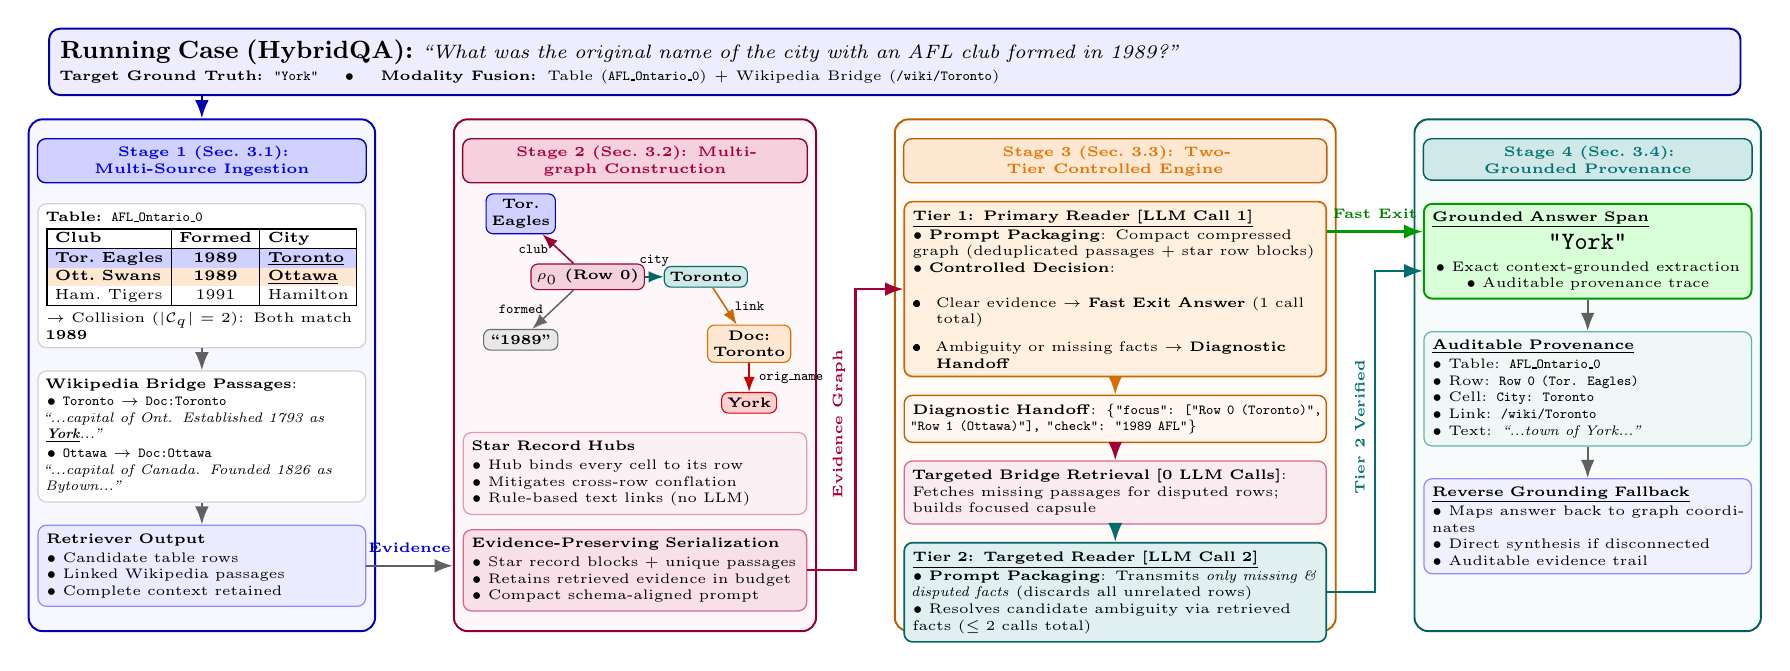
\begin{tikzpicture}[
  >=Latex,
  font=\scriptsize,
  panel/.style={draw=#1!75!black, fill=#1!3, rounded corners=5pt, line width=0.7pt},
  titlebar/.style={fill=#1!18, draw=#1!75!black, line width=0.5pt, rounded corners=3pt, font=\bfseries\fontsize{5.2pt}{6.2pt}\selectfont, text=#1!90!black, align=center, inner sep=2.5pt, minimum height=4.2mm},
  subcard/.style={draw=gray!35, fill=white, rounded corners=3pt, align=left, inner sep=3pt, font=\tiny, line width=0.45pt},
  llmcard/.style={draw=#1!80!black, fill=#1!12, rounded corners=3pt, align=left, inner sep=3pt, font=\tiny, line width=0.6pt},
  flow/.style={->, line width=0.8pt, draw=gray!75!black},
  flow_teal/.style={->, line width=0.85pt, draw=teal!85!black},
  flow_green/.style={->, line width=0.85pt, draw=green!60!black},
  flow_orange/.style={->, line width=0.8pt, draw=orange!85!black},
  flow_purple/.style={->, line width=0.8pt, draw=purple!85!black},
  knode/.style={draw=#1!85!black, fill=#1!18, rounded corners=2.5pt, inner sep=2pt, font=\tiny\bfseries, align=center},
  kedge/.style={->, line width=0.55pt, draw=#1!80!black, font=\tiny}
]

% ========================================================
% TOP BANNER: RUNNING USE CASE QUESTION
% Total width: 22.0cm, Center: 11.00
% ========================================================
\node[draw=blue!65!black, fill=blue!7, rounded corners=4pt, line width=0.7pt, text width=21.2cm, inner sep=4pt, align=left] (q_box) at (11.00, 3.98) {
  \textbf{\small Running Case (HybridQA):} \textit{``What was the original name of the city with an AFL club formed in 1989?''} \\
  \tiny \textbf{Target Ground Truth:} \texttt{"York"} \quad $\bullet$ \quad \textbf{Modality Fusion:} Table (\texttt{AFL\_Ontario\_0}) $+$ Wikipedia Bridge (\texttt{/wiki/Toronto})
};

% ========================================================
% STAGE 1: MULTI-SOURCE EVIDENCE INGESTION (Sec. 3.1)
% Panel: height 6.5cm, Center Y: -0.00, Top: 3.25, Bot: -3.25
% ========================================================
\node[panel=blue, minimum width=4.4cm, minimum height=6.5cm] (panel1) at (2.20, 0.00) {};
\node[titlebar=blue, text width=4.0cm, anchor=north] (t1) at ([yshift=-2.5mm]panel1.north) {Stage 1 (Sec.~3.1): Multi-Source Ingestion};

\node[subcard, text width=3.95cm, anchor=north] (table_box) at ([yshift=-2.5mm]t1.south) {
  {\fontsize{5pt}{6pt}\selectfont
  \textbf{Table: \texttt{AFL\_Ontario\_0}} \\[0.5mm]
  \resizebox{\linewidth}{!}{%
  \renewcommand{\arraystretch}{1.05}%
  \setlength{\tabcolsep}{2.5pt}%
  \begin{tabular}{|l|c|l|}
    \hline
    \textbf{Club} & \textbf{Formed} & \textbf{City} \\
    \hline
    \rowcolor{blue!18} \textbf{Tor.\ Eagles} & \textbf{1989} & \textbf{\underline{Toronto}} \\
    \rowcolor{orange!18} \textbf{Ott.\ Swans} & \textbf{1989} & \textbf{\underline{Ottawa}} \\
    Ham.\ Tigers & 1991 & Hamilton \\
    \hline
  \end{tabular}%
  }\\[0.5mm]
  $\rightarrow$ Collision ($|\mathcal{C}_q|=2$): Both match \textbf{1989}
  \par}
};

\node[subcard, text width=3.95cm, anchor=north] (link_box) at ([yshift=-2.8mm]table_box.south) {
  {\fontsize{5pt}{6pt}\selectfont
  \textbf{Wikipedia Bridge Passages}: \\
  $\bullet$ \texttt{Toronto} $\rightarrow$ \texttt{Doc:Toronto} \\
  \textit{``...capital of Ont. Established 1793 as \textbf{\underline{York}}...''} \\[0.3mm]
  $\bullet$ \texttt{Ottawa} $\rightarrow$ \texttt{Doc:Ottawa} \\
  \textit{``...capital of Canada. Founded 1826 as Bytown...''}
  \par}
};

\node[subcard, text width=3.95cm, fill=blue!8, draw=blue!45, anchor=north] (retr_summary) at ([yshift=-2.8mm]link_box.south) {
  {\fontsize{5pt}{6pt}\selectfont
  \textbf{Retriever Output} \\[0.3mm]
  $\bullet$ Candidate table rows \\
  $\bullet$ Linked Wikipedia passages \\
  $\bullet$ Complete context retained
  \par}
};

\draw[flow] (table_box.south) -- (link_box.north);
\draw[flow] (link_box.south) -- (retr_summary.north);

% ========================================================
% STAGE 2: SCHEMA-PRESERVING MULTIGRAPH (Sec. 3.2)
% Panel: height 6.5cm, Center Y: -0.00
% ========================================================
\node[panel=purple, minimum width=4.6cm, minimum height=6.5cm] (panel2) at (7.70, 0.00) {};
\node[titlebar=purple, text width=4.2cm, anchor=north] (t2) at ([yshift=-2.5mm]panel2.north) {Stage 2 (Sec.~3.2): Multigraph Construction};

% Graph nodes (star topology centered at \rho_0)
\node[knode=purple] (rec_node) at (7.10, 1.25) {$\rho_0$ (Row 0)};
\node[knode=blue] (ent_club) at (6.25, 2.05) {Tor.\\Eagles};
\node[knode=gray] (lit_year) at (6.25, 0.45) {``1989''};
\node[knode=teal] (ent_city) at (8.60, 1.25) {Toronto};
\node[knode=orange] (doc_node) at (9.15, 0.40) {Doc:\\Toronto};
\node[knode=red] (ans_node_g) at (9.15, -0.35) {York};

% Graph edges (outward rays from star hub \rho_0, then cross-modal bridge)
\draw[kedge=purple] (rec_node) -- node[left, font=\tiny] {\texttt{club}} (ent_club);
\draw[kedge=gray] (rec_node) -- node[left, font=\tiny] {\texttt{formed}} (lit_year);
\draw[kedge=teal] (rec_node) -- node[above, font=\tiny] {\texttt{city}} (ent_city);
\draw[kedge=orange] (ent_city) -- node[right, font=\tiny] {\texttt{link}} (doc_node);
\draw[kedge=red] (doc_node) -- node[right, font=\tiny] {\texttt{orig\_name}} (ans_node_g);

\node[subcard, text width=4.15cm, fill=purple!6, draw=purple!40, anchor=north] (centroid_box) at (7.70, -0.72) {
  {\fontsize{5pt}{6pt}\selectfont
  \textbf{Star Record Hubs} \\[0.3mm]
  $\bullet$ Hub binds every cell to its row \\
  $\bullet$ Mitigates cross-row conflation \\
  $\bullet$ Rule-based text links (no LLM)
  \par}
};

\node[subcard, text width=4.15cm, fill=purple!12, draw=purple!60, anchor=north] (path_box) at ([yshift=-1.8mm]centroid_box.south) {
  {\fontsize{5pt}{6pt}\selectfont
  \textbf{Evidence-Preserving Serialization} \\[0.3mm]
  $\bullet$ Star record blocks $+$ unique passages \\
  $\bullet$ Retains retrieved evidence in budget \\
  $\bullet$ Compact schema-aligned prompt
  \par}
};

% ========================================================
% STAGE 3: TWO-TIER CONTROLLED REASONING ENGINE (Sec. 3.3)
% Panel: height 6.5cm, Center Y: -0.00
% ========================================================
\node[panel=orange, minimum width=5.6cm, minimum height=6.5cm] (panel3) at (13.80, 0.00) {};
\node[titlebar=orange, text width=5.2cm, anchor=north] (t3) at ([yshift=-2.5mm]panel3.north) {Stage 3 (Sec.~3.3): Two-Tier Controlled Engine};

% Tier 1 LLM Card
\node[llmcard=orange, text width=5.15cm, anchor=north] (l1_box) at ([yshift=-2.2mm]t3.south) {
  {\fontsize{5pt}{6pt}\selectfont
  \textbf{\underline{Tier 1: Primary Reader [LLM Call 1]}} \\[0.3mm]
  $\bullet$ \textbf{Prompt Packaging}: Compact compressed graph (deduplicated passages $+$ star row blocks) \\
  $\bullet$ \textbf{Controlled Decision}:
  \vspace{-0.5mm}
  \begin{itemize}[leftmargin=3mm]
    \setlength{\itemsep}{0pt}
    \item Clear evidence $\rightarrow$ \textbf{Fast Exit Answer} (1 call total)
    \item Ambiguity or missing facts $\rightarrow$ \textbf{Diagnostic Handoff}
  \end{itemize}
  \par}
};

% Diagnostic Packet Box
\node[subcard, text width=5.15cm, fill=orange!6, draw=orange!75!black, line width=0.5pt, anchor=north] (handoff_box) at ([yshift=-2.2mm]l1_box.south) {
  {\fontsize{5pt}{6pt}\selectfont
  \textbf{Diagnostic Handoff}: \texttt{\{"focus": ["Row 0 (Toronto)", "Row 1 (Ottawa)"], "check": "1989 AFL"\}}
  \par}
};

% Targeted Bridge Re-retrieval
\node[subcard, text width=5.15cm, fill=purple!8, draw=purple!60, anchor=north] (ret_box) at ([yshift=-2.2mm]handoff_box.south) {
  {\fontsize{5pt}{6pt}\selectfont
  \textbf{Targeted Bridge Retrieval [0 LLM Calls]}: \\
  Fetches missing passages for disputed rows; builds focused capsule
  \par}
};

% Tier 2 LLM Card
\node[llmcard=teal, text width=5.15cm, anchor=north] (l2_box) at ([yshift=-2.2mm]ret_box.south) {
  {\fontsize{5pt}{6pt}\selectfont
  \textbf{\underline{Tier 2: Targeted Reader [LLM Call 2]}} \\[0.3mm]
  $\bullet$ \textbf{Prompt Packaging}: Transmits \emph{only missing \& disputed facts} (discards all unrelated rows) \\
  $\bullet$ Resolves candidate ambiguity via retrieved facts ($\le 2$ calls total)
  \par}
};

\draw[flow_orange] (l1_box.south) -- (handoff_box.north);
\draw[flow_purple] (handoff_box.south) -- (ret_box.north);
\draw[flow_teal] (ret_box.south) -- (l2_box.north);

% ========================================================
% STAGE 4: GROUNDED GENERATION & PROVENANCE AUDIT (Sec. 3.4)
% Panel: height 6.5cm, Center Y: -0.00
% ========================================================
\node[panel=teal, minimum width=4.4cm, minimum height=6.5cm] (panel4) at (19.80, 0.00) {};
\node[titlebar=teal, text width=4.0cm, anchor=north] (t4) at ([yshift=-2.5mm]panel4.north) {Stage 4 (Sec.~3.4): Grounded Provenance};

% Answer box aligned with l1_box center vertically!
\node[subcard, text width=3.95cm, fill=green!15, draw=green!60!black, line width=0.7pt, anchor=north] (ans_box) at ([yshift=-2.8mm]t4.south) {
  {\fontsize{5pt}{6pt}\selectfont
  \textbf{\underline{Grounded Answer Span}} \\[0.5mm]
  \centering{\textbf{\small \texttt{"York"}}}\\[0.6mm]
  $\bullet$ Exact context-grounded extraction \\
  $\bullet$ Auditable provenance trace
  \par}
};

\node[subcard, text width=3.95cm, fill=teal!6, draw=teal!60, anchor=north] (prov_box) at ([yshift=-4.0mm]ans_box.south) {
  {\fontsize{5pt}{6pt}\selectfont
  \textbf{\underline{Auditable Provenance}} \\[0.3mm]
  $\bullet$ Table: \texttt{AFL\_Ontario\_0} \\
  $\bullet$ Row: \texttt{Row 0 (Tor. Eagles)} \\
  $\bullet$ Cell: \texttt{City: Toronto} \\
  $\bullet$ Link: \texttt{/wiki/Toronto} \\
  $\bullet$ Text: \textit{``...town of York...''}
  \par}
};

\node[subcard, text width=3.95cm, fill=blue!6, draw=blue!45, anchor=north] (rev_box) at ([yshift=-4.0mm]prov_box.south) {
  {\fontsize{5pt}{6pt}\selectfont
  \textbf{\underline{Reverse Grounding Fallback}} \\[0.3mm]
  $\bullet$ Maps answer back to graph coordinates \\
  $\bullet$ Direct synthesis if disconnected \\
  $\bullet$ Auditable evidence trail
  \par}
};

\draw[flow] (ans_box.south) -- (prov_box.north);
\draw[flow] (prov_box.south) -- (rev_box.north);

% ========================================================
% INTER-STAGE CONNECTORS (Rotated Vertical Labels to Prevent Overlap)
% ========================================================
% Top question to Stage 1
\draw[flow, draw=blue!70!black] (q_box.south -| panel1.north) -- (panel1.north);

% Stage 1 -> Stage 2: rotated vertical label in corridor
\draw[flow] (retr_summary.east) -- node[midway, above=1pt, font=\fontsize{4.8pt}{5.8pt}\selectfont\bfseries, text=blue!85!black] {Evidence} (panel2.west |- retr_summary.east);

% Stage 2 -> Stage 3: vertical segment with vertical label in corridor
\draw[flow, draw=purple!85!black] (path_box.east) -- (10.50, 0 |- path_box.east) -- node[midway, rotate=90, above=2pt, font=\tiny\bfseries, text=purple!90!black] {Evidence Graph} (10.50, 0 |- l1_box.west) -- (l1_box.west);

% Stage 3 -> Stage 4: Branch 1: Fast Exit (strictly horizontal)
\coordinate (fast_exit_end) at ([yshift=2.5mm]ans_box.west);
\coordinate (fast_exit_start) at (l1_box.east |- fast_exit_end);
\draw[flow_green] (fast_exit_start) -- node[midway, above=1pt, font=\fontsize{4.8pt}{5.8pt}\selectfont\bfseries, text=green!50!black] {Fast Exit} (fast_exit_end);

% Stage 3 -> Stage 4: Branch 2: Tier 2 Verified (strictly orthogonal Manhattan routing)
\coordinate (t2_end) at ([yshift=-2.5mm]ans_box.west);
\coordinate (t2_corner2) at (17.10, 0 |- t2_end);
\coordinate (t2_corner1) at (17.10, 0 |- l2_box.east);
\draw[flow_teal] (l2_box.east) -- (t2_corner1) -- node[pos=0.5, rotate=90, above=1.5pt, font=\fontsize{4.8pt}{5.8pt}\selectfont\bfseries, text=teal!90!black] {Tier 2 Verified} (t2_corner2) -- (t2_end);

\end{tikzpicture}
}
\Description{End-to-end architecture of QEG-RAG illustrating the four stages: Multi-Source Evidence Ingestion, Schema-Preserving Multigraph Construction, Two-Tier Controlled Reasoning Engine, and Grounded Provenance Audit.}
\vspace{2.5mm}
\caption{End-to-end architecture of QEG-RAG. (Sec.~\ref{sec:method-retrieval}) Multi-Source Evidence Ingestion retrieves relevant table rows and linked passages. (Sec.~\ref{sec:method-kg}) Schema-Preserving Multigraph Construction builds star record hubs and text relations without LLMs. (Sec.~\ref{sec:method-engine}) Two-Tier Controlled Reasoning Engine: Tier~1 reads the compressed evidence graph; unambiguous cases exit immediately in one call, while ambiguous collisions trigger a diagnostic handoff and targeted bridge retrieval for conclusive resolution in Tier~2. (Sec.~\ref{sec:method-answer}) Grounded Generation and Provenance Audit outputs verified spans with full attribution traces.}
\vspace{-2mm}
\label{fig:pipeline}
\end{figure}


To systematically resolve these challenges, QEG-RAG orchestrates four cohesive stages: Stage~1 ingests multimodal evidence; Stage~2 constructs an LLM-free schema-preserving multigraph enforcing tabular semantics ($\rho_i$); Stage~3 executes diagnostic-driven retrieval feedback over a bounded two-tier execution protocol ($\mathcal{S}_{\min}$); and Stage~4 conducts grounded generation with provenance auditing.

\paragraph{Problem Formulation and Graph Representation.}
\label{sec:formulation}
We formulate the task of multi-hop question answering over heterogeneous tabular and textual knowledge sources. An input instance is defined as a tuple $\mathcal{I} = (q, T, \mathcal{D}_T)$, where $q$ is a natural language question; $T = (C, R)$ is a semi-structured table comprising ordered headers $C = (c_1, \dots, c_m)$ and rows $R = \{r_1, \dots, r_n\}$ with discrete cells $v_{i,j}$; and $\mathcal{D}_T = \{d_1, \dots, d_K\}$ is the corpus of external text passages associated with $T$, where cell entities connect to external passages via relational mappings $\ell(v_{i,j}) \rightarrow d_k$. The objective is to extract the grounded answer span $a^* \in \mathcal{A}$ along with verifiable provenance traces, where $a^*$ may reside as a table cell ($a^* = v_{i,j}$) or as an unstructured text span within a linked passage ($a^* \subset d_k$).

\paragraph{Online Evidence Multigraph Representation.}
Unlike persistent knowledge base settings that depend on static global entity graphs, table--text RAG requires synthesizing unstructured text with tabular structures on-the-fly. For each query $q$, we dynamically instantiate a bounded, query-specific directed multigraph $G_q = (V_q, E_q, \psi_V, \psi_E)$ whose node and edge sets are partitioned as:
\begin{equation}
\label{eq:graph-partition}
V_q = V_{\text{ent}} \cup V_{\text{rec}} \cup V_{\text{lit}}, \qquad
E_q = E_{\text{rec}} \cup E_{\text{attr}} \cup E_{\text{link}} \cup E_{\text{text}}.
\end{equation}
The node partition divides vertices by semantic abstraction:
\begin{itemize}[leftmargin=1.5em]
    \item $V_{\text{ent}}$: Named entity mentions extracted from linked table cells or passage text spans.
    \item $V_{\text{rec}} = \{\rho_i \mid r_i \in R\}$: Local star-topology record hub centroids, where each node $\rho_i = \texttt{table:}T\texttt{:row:}i$ uniquely anchors and binds all cell attributes of row $r_i$ to mitigate cross-row attribute conflation.
    \item $V_{\text{lit}}$: Unlinked literal values (e.g., numbers, scores, dates, unlinked strings).
\end{itemize}
The edge set $E_q$ consists of directed relational facts $e = (h, r, t, \pi)$, where $h, t \in V_q$, $r$ is a normalized predicate, and $\pi = (\text{src\_id}, \text{row\_idx}, \text{col\_name})$ stores source provenance:
\begin{itemize}[leftmargin=1.5em]
    \item $E_{\text{rec}} = \{ (u_i, \texttt{has\_record}, \rho_i) \}$: Structural edges connecting row subject entity $u_i$ to its centroid hub $\rho_i$.
    \item $E_{\text{attr}} = \{ (\rho_i, \operatorname{norm}(H_j), v_{i,j}) \}$: Schema-level attribute edges from centroid $\rho_i$ to column cell values $v_{i,j}$.
    \item $E_{\text{link}} = \{ (v_{i,j}, \texttt{linked\_passage}, d_k) \}$: Cross-modal linking edges connecting candidate cells to associated external text passages.
    \item $E_{\text{text}}$: Intra-passage relational triples extracted from retrieved passage sentences.
\end{itemize}

\paragraph{Schema-Preservation and Non-Conflation Property.}
We define the intra-row star subgraph $\mathcal{G}^*(\rho_i) \subset G_q$ for row $r_i$ as:
\begin{equation}
\label{eq:star-subgraph}
\begin{aligned}
\mathcal{G}^*(\rho_i) = \Big( &\{\rho_i, u_i\} \cup \{v_{i,j}\}_{j=1}^m, \\
&\{(u_i, \texttt{has\_record}, \rho_i)\} \cup \{(\rho_i, \operatorname{norm}(H_j), v_{i,j})\}_{j=1}^m \Big).
\end{aligned}
\end{equation}
By construction, for any distinct table rows $r_i, r_{i'} \in R$ ($i \neq i'$), their star centroids are strictly disjoint: $V(\mathcal{G}^*(\rho_i)) \cap V(\mathcal{G}^*(\rho_{i'})) \cap V_{\text{rec}} = \emptyset$. Consequently, every cell value $v_{i,j}$ maintains a unique 1-hop connection to its parent record centroid $\rho_i$, mitigating horizontal cross-row attribute conflation across symmetric candidate rows without requiring destructive graph pruning.

Once question answering concludes, the dynamic multigraph $G_q$ is discarded, incurring zero persistent graph database index overhead. Throughout this section, we illustrate QEG-RAG via the running HybridQA example depicted in Fig.~\ref{fig:pipeline}: \textit{``What was the original name of the city with an AFL club formed in 1989?''} (ground truth: \texttt{York}).

\subsection{Stage 1: Multi-Source Evidence Ingestion}
\label{sec:method-retrieval}
Given an input table and an associated corpus of external text passages, retrieval operates dynamically at query time:
\begin{itemize}[leftmargin=1.5em]
    \item \emph{Coarse row retrieval and query anchoring}: A lexical retriever indexes table rows with respect to question $q$. A deterministic query anchor inspects $q$ for ordinal constraints (e.g., ``second'', ``last'') and exact schema constraints (column header mentions, numerical filters), selecting top-$k_1$ rows. In Fig.~\ref{fig:pipeline}, the constraint ``formed in 1989'' anchors both Row~0 (\texttt{Tor. Eagles}, Toronto) and Row~1 (\texttt{Ott. Swans}, Ottawa), exposing a candidate collision ($|\mathcal{C}_q| = 2$).
    \item \emph{Passage expansion via cross-modal linking}: Rather than retrieving entire document corpora indiscriminately, the passage expander resolves relevant external text passages linked to candidate entities in the top-$k_1$ retrieved rows (via hyperlinks or entity linking) up to a budget of $k_2$ passages. In Fig.~\ref{fig:pipeline}, candidate bridge cells link to \texttt{Doc:Toronto} and \texttt{Doc:Ottawa}.
\end{itemize}

\enlargethispage{2.5\baselineskip}
\subsection{Stage 2: Schema-Preserving Multigraph Construction}
\label{sec:method-kg}
Using the retrieved rows and passages, the system dynamically instantiates the multigraph $G_q=(V_q, E_q)$ without LLM calls:
\begin{itemize}[leftmargin=1.5em]
    \item \emph{Centroid bindings}: For each candidate row $i$, local record centroid $\rho_i \in V_{\text{rec}}$ binds row attributes via $E_{\text{rec}}$ and $E_{\text{attr}}$ (Eq.~\ref{eq:star-subgraph}).
    \item \emph{Cross-modal bridging and deterministic text relation extraction}: Edges $E_{\text{link}}$ connect table cell entities to external passage nodes (e.g., linking cell \texttt{Toronto} to passage \texttt{Doc:Toronto}). Rule-based text triples $E_{\text{text}}$ are extracted deterministically (0 LLM calls) via dependency parse patterns: copular constructions (``[Subject] is/was [Attribute]''), parenthetical appositives (e.g., ``York (1793)''), and anchor hyperlinks, directly linking entities to textual attributes without LLM extraction latency or relational drift.
\end{itemize}

\subsection{Stage 3: Two-Tier Controlled Reasoning Engine}
\label{sec:method-engine}

% Figure 3 removed (subsumed by Fig 2)

QEG-RAG resolves the operational dilemma between destructive graph pruning and unbounded agentic loops. As illustrated in Fig.~\ref{fig:pipeline} (Stage~3), the reasoning engine coordinates four transparent steps across two strictly bounded execution tiers:

\paragraph{Tier 1: Primary Reader and Evidence-Preserving Graph Packaging (First LLM Call).}
Tier~1 evaluates the initial multimodal evidence graph without destructive pruning. To supply complete evidence within context limits, we formulate a compressed prompt packaging protocol:
\begin{equation}
\label{eq:compression}
\mathcal{X}^*(G_q) = \operatorname{Enc}_{\text{table}}\left(\{\mathcal{G}^*(\rho_i)\}_{i=1}^{k_1}\right) \;\parallel\; \operatorname{Enc}_{\text{text}}(\mathcal{D}_{\text{unique}}),
\end{equation}
where table rows are serialized into structured star centroid blocks preserving hierarchical column predicates, while external passages are deduplicated, indexed once by source identifier, and ordered along relevant cross-modal traversal hints to guide sequential model attention without heuristic filtering. This schema-aligned prompt compression reduces textual redundancy while retaining retrieved evidence facts within the context budget.

\enlargethispage{4.5\baselineskip}
The primary reader language model $\mathcal{M}$ is then invoked over prompt $\mathcal{X}_1 = (q, \mathcal{X}^*(G_q))$. Let $\mathcal{C}_q \subseteq V_{\text{rec}}$ denote candidate record centroids satisfying question filter constraints (e.g., matching qualifying dates or relational attributes). When evaluating $\mathcal{X}_1$, the model executes an adaptive diagnostic audit:
\begin{itemize}[leftmargin=1.5em]
    \item \emph{Fast Exit (Determined State)}: If candidate evidence is unambiguous ($|\mathcal{C}_q| = 1$) and required bridge evidence is fully present within $G_q$, the model directly extracts the verified answer span, $a^* = \arg\max_{a \in \mathcal{A}} P_{\mathcal{M}}(a \mid \mathcal{X}_1)$, concluding execution in a single LLM call ($\approx 80\%$ of queries).
    \item \emph{Diagnostic Handoff (Under-Determined State)}: If structural ambiguity or candidate collisions arise ($|\mathcal{C}_q| > 1$, e.g., competing clubs \texttt{Tor. Eagles} (Toronto) vs.\ \texttt{Ott. Swans} (Ottawa) both satisfying \texttt{Formed = 1989} while external bridge passage evidence is incomplete), the model defers ungrounded guessing. Instead, it emits a structured diagnostic packet $\mathcal{D} = (\mathcal{C}_{\text{focus}}, \, \beta, \, \psi_{\text{check}})$ (Handoff~$\mathcal{D}$), specifying the disputed candidate rows $\mathcal{C}_{\text{focus}}$, blocker category $\beta$, and unresolved factual predicate $\psi_{\text{check}}$.
\end{itemize}

\paragraph{Diagnostic Handoff and Targeted Bridge Augmentation.}
Upon receiving diagnostic packet $\mathcal{D}$, an automated retriever (0 LLM calls) executes targeted bridge search: it fetches missing bridge passages $\Delta\mathcal{D}$ (e.g., \texttt{Doc:Toronto} and \texttt{Doc:Ottawa}) exclusively for disputed candidate rows $\mathcal{C}_{\text{focus}}$:
\begin{equation}
\label{eq:targeted-retrieval}
\Delta \mathcal{D} = \bigcup_{c \in \mathcal{C}_{\text{focus}}} \left( \ell(c) \setminus \mathcal{D}_{\text{current}} \right),
\end{equation}
enforcing a symmetric per-candidate retrieval quota to maintain evidentiary balance.

\paragraph{Tier 2: Targeted Reader and State Capsule Packaging (Second LLM Call).}
Crucially, rather than re-transmitting the broad multigraph, the engine executes deterministic graph compression by pruning non-competing candidates (achieving $\approx 85\%$ size reduction), packaging \emph{exclusively the missing and disputed evidence} into a minimal state capsule $\mathcal{S}_{\min}$:
\begin{equation}
\label{eq:l2-capsule}
\mathcal{S}_{\min} = \left( q, \, \psi_{\text{check}}, \, \{ \mathcal{G}^*(\rho_c) \}_{c \in \mathcal{C}_{\text{focus}}}, \, \Delta \mathcal{D} \right).
\end{equation}
By filtering out non-competing candidates and retaining only disputed record centroids and newly fetched bridge passages $\Delta \mathcal{D}$ (\texttt{Doc:Toronto}), $\mathcal{S}_{\min}$ reduces context dilution. In Tier~2, the language model $\mathcal{M}$ resolves ambiguity directly against factual bridge evidence in a targeted second call:
\begin{equation}
a^* = \arg\max_{a \in \mathcal{A}} P_{\mathcal{M}}(a \mid \mathcal{S}_{\min}),
\end{equation}
producing the verified answer span (e.g., \texttt{"York"}) with verifiable provenance traces (Row~0 $\to$ \texttt{Doc:Toronto} $\to$ \texttt{town of York (1793)}) within at most two LLM calls.

\subsection{Stage 4: Grounded Generation and Structural Provenance}
\label{sec:method-answer}
QEG-RAG enforces grounding through an explicit structural mechanism: rather than unconstrained text generation, the final output is bound to the multigraph via an inspectable provenance homomorphism $\pi: a^* \rightarrow E_q^*$. This mapping anchors the extracted answer span directly to traversed source coordinates: specific table cells (\texttt{AFL\_Ontario\_0:row:0}), bridge entity URLs (\texttt{/wiki/Toronto}), and supporting passage excerpts (\texttt{town of York (1793)}). To ensure evidentiary fidelity, an automated verification check confirms that the synthesized answer span is factually contained within the resolved evidence nodes, flagging hallucinated citations. Under our strict in-context evaluation protocol, language models are constrained to synthesize answers exclusively from retrieved evidence; downstream gains in EM and $\text{F}_1$ confirm that structural graph serialization enables models to locate ground-truth evidence factually, rather than suffering from attention dispersion across flat serializations. If graph search disconnects, \emph{reverse grounding} synthesizes directly over retrieved context and maps the extracted span back onto $G_q$.

\section{Experimental Protocol}
\label{sec:experiments}

\subsection{Benchmark Datasets and Evaluation Protocol}
We evaluate across two challenging multi-hop table--text benchmarks ($N=1{,}500$ each, sampled from official development splits following~\cite{agarwal2025hybrid}): (1)~\emph{HybridQA}~\cite{hybridqa}, evaluating reasoning over Wikipedia tables aligned with hyperlinked passages; and (2)~\emph{OTT-QA}~\cite{chen2021ottqa}, evaluating open table-and-text retrieval and question answering where tables and text spans must be jointly fetched. Both benchmarks require integrating semi-structured table cells with unstructured passages, providing a realistic testbed for evaluating cross-modal multi-hop reasoning and targeted diagnostic disambiguation when candidate ambiguities arise.

\paragraph{Evaluation Scope.}
Unlike supervised models (e.g., MuGER$^2$~\cite{wang2022muger2}, S3HQA~\cite{lei2023s3hqa}) that fine-tune millions of parameters on benchmark-specific training instances, QEG-RAG operates strictly in the training-free, zero-shot in-context RAG regime (0 training examples, 0 updated weights) under standardized retrieval pools ($k_1=5, k_2=3$) and context budgets ($24{,}000$ characters). We report Exact Match (EM, measuring exact normalized string match) and token-level macro $\text{F}_1$ (evaluating harmonic token overlap following standard QA protocols), along with average LLM calls. Crucially, all reported metrics in Table~\ref{tab:main-results} are computed unconditionally across the full population ($N=1{,}500$ per benchmark): empty model responses or ungrounded abstentions are strictly penalized and scored as 0 rather than excluded from the denominator.

\begin{table}[t]
\caption{Comprehensive comparative evaluation of native reasoning models across multi-hop table--text benchmarks under strict context grounding ($k_1=5, k_2=3$, 24k context budget, $N=1{,}500$ per benchmark, unconditional metrics with unextracted/empty answers scored as 0; $^*$adapted graph-pruning protocol~\cite{agarwal2025hybrid}).}
\label{tab:main-results}
\vspace{1.5mm}
\centering
\scriptsize
\renewcommand{\arraystretch}{0.88}
\setlength{\tabcolsep}{7pt}
\begin{tabular}{@{}lllrrr@{}}
\toprule
Dataset & Model & Method & EM (\%) & $\text{F}_1$ (\%) & Calls \\
\midrule
\multirow{10}{*}{HybridQA} & \multirow{5}{*}{GPT-OSS 20B}  
  & Direct LLM               & 45.73 & 54.25 & 1.00 \\
& & ODYSSEY$^*$~\cite{agarwal2025hybrid} & 32.80 & 39.98 & 5.39 \\
& & Flat Graph RAG           & 31.80 & 37.92 & 1.00 \\
& & Pruned Subgraph RAG      & 10.87 & 12.53 & 1.00 \\
& & \textbf{QEG-RAG (Ours)}  & \textbf{53.07} & \textbf{66.45} & 1.23 \\
\cmidrule{2-6}
& \multirow{5}{*}{GPT-OSS 120B} 
  & Direct LLM               & 56.20 & 65.62 & 1.00 \\
& & ODYSSEY$^*$~\cite{agarwal2025hybrid} & 37.80 & 45.17 & 5.38 \\
& & Flat Graph RAG           & 33.93 & 39.80 & 1.00 \\
& & Pruned Subgraph RAG      & 13.07 & 15.13 & 1.00 \\
& & \textbf{QEG-RAG (Ours)}  & \textbf{59.27} & \textbf{70.70} & 1.20 \\
\midrule
\multirow{10}{*}{OTT-QA}   & \multirow{5}{*}{GPT-OSS 20B}  
  & Direct LLM               & 50.80 & 57.70 & 1.00 \\
& & ODYSSEY$^*$~\cite{agarwal2025hybrid} & 37.47 & 43.66 & 5.44 \\
& & Flat Graph RAG           & 40.87 & 46.35 & 1.00 \\
& & Pruned Subgraph RAG      & 9.40  & 10.39 & 1.00 \\
& & \textbf{QEG-RAG (Ours)}  & \textbf{55.60} & \textbf{67.59} & 1.24 \\
\cmidrule{2-6}
& \multirow{5}{*}{GPT-OSS 120B} 
  & Direct LLM               & 60.40 & 67.93 & 1.00 \\
& & ODYSSEY$^*$~\cite{agarwal2025hybrid} & 41.73 & 47.96 & 5.48 \\
& & Flat Graph RAG           & 42.27 & 47.58 & 1.00 \\
& & Pruned Subgraph RAG      & 13.20 & 14.88 & 1.00 \\
& & \textbf{QEG-RAG (Ours)}  & \textbf{62.93} & \textbf{73.03} & 1.22 \\
\bottomrule
\end{tabular}
\vspace{1.0mm}
\end{table}

\subsection{Baselines and Experimental Settings}
\paragraph{In-Context Reasoning Condition.}
To ensure consistent and comparable evaluation, all baselines and our method operate under a strict in-context reasoning condition: models are explicitly instructed to reason exclusively within the provided context and are forbidden from relying on external or pre-training parametric knowledge without factual grounds. We exclude agentic online KG frameworks (HydraRAG~\cite{tan2025hydrarag}, ToG-3~\cite{wu2025tog3}) as direct baselines because they deploy unconstrained multi-agent LLM loops requiring 10--30+ LLM calls per query with open-ended exploration, violating our bounded operational protocol ($\le 2$ calls) and latency-sensitive query-time constraints. For ODYSSEY~\cite{agarwal2025hybrid}, we evaluate an adapted protocol ($\text{ODYSSEY}^*$) under standardized retrieval ($k_1=5, k_2=3$) and strict in-context reasoning. While the original ODYSSEY pipeline employs specialized dense embedding models (INSTRUCTOR-XL) and unconstrained parametric prompting (where the LLM can freely compensate for pruned evidence through pre-trained memory), $\text{ODYSSEY}^*$ isolates the published query-time entity graph construction and question-token similarity pruning protocol under strict context grounding: models are forbidden from parametric hallucination when context is incomplete.

\paragraph{Paradigms and Configurations.}
We evaluate across: (1)~\emph{Primary Reasoning Models}: GPT-OSS 20B and 120B with native reasoning tokens; and (2)~\emph{Non-Reasoning LLMs}: Qwen 122B (\texttt{Qwen3.5-122B-A10B}, 10B active MoE parameters, evaluated with test-time reasoning disabled via \texttt{enable\_thinking=false}) on OTT-QA to test neuro-symbolic scaffolding without test-time reasoning tokens.
Under an identical context budget ($24{,}000$ characters), we compare five configurations:
(1)~\emph{Direct LLM}: standard RAG over linearized tables and text;
(2)~\emph{ODYSSEY$^*$}~\cite{agarwal2025hybrid}: zero-shot hybrid graph-pruning protocol adapted from~\cite{agarwal2025hybrid} under strict in-context grounding;
(3)~\emph{Flat Graph RAG}: unpruned multigraph serialized without structured evidence packaging;
(4)~\emph{Pruned Subgraph RAG}: hard-filtered subgraph keeping only top-ranked entity triples; and
(5)~\emph{QEG-RAG (Ours)}: complete framework integrating compact prompt compression (retaining retrieved evidence within budget), schema-preserving star centroids, and the bounded two-tier diagnostic reasoning engine.

\section{Results and In-Depth Analysis}
\label{sec:results}
\enlargethispage{4.5\baselineskip}
To systematically assess the empirical performance and architectural mechanisms of QEG-RAG, we formulate and address five key research questions grounded in quantitative benchmark evidence:

\paragraph{RQ1 (Main Benchmark Grounding Performance):}
\emph{Under strict context grounding and prevalent retrieval ambiguities, does QEG-RAG achieve higher grounding accuracy and mitigate ungrounded failures across heterogeneous benchmarks compared to direct prompting and hybrid graph baselines?}

\emph{Empirical Findings}: Table~\ref{tab:main-results} reports primary results across HybridQA and OTT-QA ($N=1{,}500$ each). QEG-RAG achieves higher grounding accuracy across all models and benchmarks at only 1.20--1.24 LLM calls (vs.\ 5.38--5.48 for ODYSSEY$^*$). On HybridQA, QEG-RAG reaches 53.07\% EM / 66.45\% $\text{F}_1$ on 20B (+7.34\,pp EM over Direct LLM; +20.27\,pp over ODYSSEY$^*$) and 59.27\% EM / 70.70\% $\text{F}_1$ on 120B (+3.07\,pp over Direct LLM; +21.47\,pp over ODYSSEY$^*$, McNemar's $p < 0.001$). On open retrieval (OTT-QA), where joint table--text retrieval increases candidate collisions, it reaches 55.60\% EM / 67.59\% $\text{F}_1$ on 20B (+4.80\,pp over Direct LLM; +18.13\,pp over ODYSSEY$^*$) and 62.93\% EM / 73.03\% $\text{F}_1$ on 120B (+2.53\,pp over Direct LLM; +21.20\,pp over ODYSSEY$^*$).

\emph{In-Depth Diagnostic Analysis}: Auditing baseline outputs shows that empty responses stem from unresolvable candidate collisions under strict context grounding, while missing or detached bridge evidence induces attribute conflation (quantified further in RQ4, Table~\ref{tab:evidence-audit}): (1)~\emph{Direct LLM} linearizes tables, dissolving schema boundaries and capping EM at 45.73\%--60.40\%; (2)~\emph{Flat Graph RAG} retains triples without schema-aligned packaging, dispersing attention (31.80\%--42.27\% EM); and (3)~\emph{ODYSSEY$^*$ \& Pruned Subgraph RAG} forbid parametric guessing under our in-context condition while question-token pruning severs peripheral cross-modal links, dropping to 32.80\%--41.73\% EM (9.40\%--13.20\% for Pruned Subgraph RAG). In contrast, QEG-RAG detects collisions ($|\mathcal{C}_q| > 1$) in Tier~1 and retrieves missing bridge passages in Tier~2 within $\mathcal{S}_{\min}$ to resolve ambiguity factually (+2.53--7.34\,pp EM).

\begin{table}[t]
\caption{Cross-paradigm generalization on non-reasoning LLM (Qwen 122B, OTT-QA, $N=1{,}500$; $^*$adapted graph protocol).}
\label{tab:qwen-results}
\vspace{1.0mm}
\centering
\scriptsize
\renewcommand{\arraystretch}{0.88}
\setlength{\tabcolsep}{8pt}
\begin{tabular}{@{}lrrr@{}}
\toprule
Method & EM (\%) & $\text{F}_1$ (\%) & Calls \\
\midrule
Direct LLM                         & 29.27 & 31.52 & 1.00 \\
ODYSSEY$^*$~\cite{agarwal2025hybrid} & 5.93  & 6.99  & 6.66 \\
Flat Graph RAG                     & 9.93  & 11.00 & 1.00 \\
Pruned Subgraph                    & 1.67  & 1.89  & 1.00 \\
\textbf{QEG-RAG (Ours)}            & \textbf{33.40} & \textbf{35.30} & 1.64 \\
\bottomrule
\end{tabular}
\vspace{1.0mm}
\end{table}

\begin{table}[t]
\caption{Systematic knockout ablation study on pooled benchmark ($N=500$, GPT-OSS 120B) isolating individual QEG-RAG components.}
\label{tab:ablation}
\vspace{1.0mm}
\centering
\scriptsize
\renewcommand{\arraystretch}{0.88}
\setlength{\tabcolsep}{6pt}
\begin{tabular}{@{}llrrr@{}}
\toprule
\multicolumn{2}{@{}l}{Ablation Configuration} & EM (\%) & $\text{F}_1$ (\%) & $\Delta\text{EM}$ (pp) \\
\midrule
\multicolumn{2}{@{}l}{\textbf{Full QEG-RAG}} & \textbf{59.20} & \textbf{68.06} & \textbf{---} \\
\midrule
(1) & w/o Prompt Comp.            & 31.60 & 37.36 & $-27.60$ \\
(2) & w/o Record Nodes $\rho_i$   & 56.20 & 62.74 & $-3.00$ \\
(3) & w/o Tier-2 Evidence         & 56.00 & 63.60 & $-3.20$ \\
(4) & w/o Diagnostic Focus        & 57.80 & 65.74 & $-1.40$ \\
(5) & w/o Adaptive Tier-2         & 58.60 & 66.78 & $-0.60$ \\
\bottomrule
\end{tabular}
\vspace{1.0mm}
\end{table}

\enlargethispage{2\baselineskip}
\paragraph{RQ2 (Cross-Paradigm Generalization to Non-Reasoning LLMs):}
\emph{Can QEG-RAG generalize beyond native reasoning architectures and improve performance on standard instruction-tuned LLMs under strict grounding?}

\emph{Finding}: Table~\ref{tab:qwen-results} evaluates cross-paradigm generalization on Qwen 122B (OTT-QA) with reasoning tokens disabled (\texttt{enable\_thinking=false}). Under strict grounding, instruction-tuned LLMs struggle with multi-hop relations: Direct LLM achieves 29.27\% EM (31.52\% $\text{F}_1$), while unorganized or pruned graph baselines degrade sharply---Flat Graph RAG to 9.93\% EM, ODYSSEY$^*$ to 5.93\% EM (6.99\% $\text{F}_1$ at 6.66 calls), and Pruned Subgraph to 1.67\% EM. In comparison, QEG-RAG reaches 33.40\% EM and 35.30\% $\text{F}_1$ (+4.13\,pp EM over Direct LLM; vs.\ 5.93\% for ODYSSEY$^*$). Noticeably, Qwen averages 1.64 LLM calls (still $4.1\times$ fewer than ODYSSEY$^*$'s 6.66), higher than the 1.20--1.24 calls of native reasoning models ($\approx 80\%$ single-call Fast Exits). Lacking internal chain-of-thought verification, the model conservatively triggers the diagnostic handoff ($\mathcal{D}$) more often ($\approx 64\%$ entering Tier~2), showing that the structured multigraph and two-tier engine serve as an effective external diagnostic scaffold when test-time reasoning tokens are unavailable.



\paragraph{RQ3 (Preserving Retrieved Evidence vs.\ Destructive Pruning):}
\emph{How does retaining retrieved evidence within context limits compare against aggressive graph pruning, and why does heuristic pruning degrade multi-hop reasoning accuracy?}
\emph{Finding}: Across Tables~\ref{tab:main-results} and~\ref{tab:qwen-results}, hard graph pruning (Pruned Subgraph RAG and ODYSSEY$^*$) degrades accuracy (1.67\%--13.20\% and 5.93\%--41.73\% EM) because filtering out peripheral nodes severs multi-hop reasoning chains across heterogeneous modalities. Conversely, feeding raw unorganized graph triples (Flat Graph RAG) disperses model attention across irrelevant entities (dropping EM to 9.93\%--42.27\%). In contrast, QEG-RAG retains retrieved multigraph evidence within the context budget via compact serialization (Row~1 in Table~\ref{tab:ablation}, without which EM drops by 27.60\,pp due to context blowout), ensuring that critical cross-modal connections remain accessible for factual verification without ungrounded extrapolation.


\begin{table}[t]
\caption{Systematic evidence grounding and structural provenance fidelity audit on HybridQA ($N=500$ test instances). Conditioned on verified provenance traces, answer correctness increases significantly (+9.80\,pp, $p < 0.0001$).}
\label{tab:evidence-audit}
\vspace{1.0mm}
\centering
\scriptsize
\renewcommand{\arraystretch}{0.85}
\setlength{\tabcolsep}{7pt}
\begin{tabular}{@{}llr@{}}
\toprule
Audit Dimension & Grounding Evaluation Metric & HybridQA \\
\midrule
\multirow{3}{*}{Evidence Coverage} 
  & Evaluated Test Cohort ($N$)                         & 500 \\
  & Response Generation Rate ($N_{\text{ans}}$)           & 86.20\% (431/500) \\
  & Grounded Output Count ($a^* \in E_q^*$)             & 431 \\
\midrule
\multirow{3}{*}{Grounding Fidelity} 
  & Grounded Answer Rate (GAR)                          & \textbf{100.0\%} \\
  & Wilson 95\% Confidence Interval                     & [99.12\%, 100\%] \\
  & Hallucinated / Invalid Citations                    & 5.48\% (25/456) \\
\midrule
\multirow{4}{*}{Grounding vs.\ Accuracy} 
  & Full-Population Exact Match (Unconditional)         & 61.20\% (306/500) \\
  & Answered Exact Match (Conditioned on $N_{\text{ans}}$) & 71.00\% (306/431) \\
  & Exact Match on Verified Provenance                  & 71.00\% (306/431) \\
  & \emph{Provenance Accuracy Boost}                    & \textbf{+9.80\,pp} \\
\midrule
\multirow{2}{*}{Ambiguity Audit ($N=100$)} 
  & Verified Provenance Alignment                       & 92.00\% \\
  & Ground-Truth Bridge Entity Match                    & 89.00\% \\
\bottomrule
\end{tabular}
\vspace{1.0mm}
\end{table}

\enlargethispage{6.0\baselineskip}
\paragraph{RQ4 (Diagnostic Feedback, Bounded Execution, and Provenance Audit):}
\emph{Can two-tier diagnostics resolve retrieval collisions under bounded execution, and how does structural provenance support verified evidence grounding?} \emph{Finding}: Unlike unbounded loops (HydraRAG), QEG-RAG concludes unambiguous queries via single-call Fast Exit ($\approx 80\%$ of queries), averaging 1.20--1.24 calls (vs.\ 5.38--6.66 for ODYSSEY$^*$). On structural collisions ($|\mathcal{C}_q| > 1$), Tier~2 and diagnostic focus resolve ambiguity factually: omitting Tier~2 (Row~5) drops $\text{F}_1$ by 1.28\,pp, omitting diagnostic focus $\mathcal{C}_{\text{focus}}$ (Row~4) reduces EM by 1.40\,pp and $\text{F}_1$ by 2.32\,pp, and omitting targeted bridge evidence $\Delta\mathcal{D}$ (Row~3) reduces EM by 3.20\,pp and $\text{F}_1$ by 4.46\,pp. 

\emph{Provenance Audit and Grounding Correlation}: As summarized in Table~\ref{tab:evidence-audit}, a systematic audit across the full $N=500$ HybridQA evaluation cohort confirms high grounding fidelity: QEG-RAG achieves a Grounded Answer Rate of 100.0\% (using the binomial Wilson score interval to bound near-ceiling rates conservatively, 95\% CI: [99.12\%, 100.0\%]), with invalid citations strictly penalized and filtered out (5.48\%, 25/456 attempts). Under strict context grounding, models refrain from ungrounded guessing when evidence is missing, emitting empty responses on 13.80\% of queries (scored as 0 in unconditional EM). Importantly, grounded answers correlate directly with higher accuracy: conditioned on verified multigraph traces ($a^* \in E_q^*$), Exact Match reaches 71.00\% (+9.80\,pp higher than the unconditional full-population EM of 61.20\%, $p < 0.0001$). To assess evidentiary integrity, two independent domain annotators (co-authors blinded to method origin) audited 100 randomly sampled collision queries ($|\mathcal{C}_q| > 1$): (1)~\emph{Trace Validity} (92.0\%, with high inter-annotator agreement measured by Cohen's $\kappa = 0.86$): an answer trace is scored as valid if and only if each intermediate hop ($\text{row} \to \text{cell} \to \text{bridge} \to \text{answer}$) is strictly substantiated by factual assertions in the cited table cells and text excerpts without ungrounded extrapolation; and (2)~\emph{Bridge Alignment} (89.0\%): scored as correct if the multigraph's resolved bridge entity matches the gold Wikipedia hyperlink specified in HybridQA ground truth (adjudicating discrepancies by consensus).

\paragraph{RQ5 (Preservation of Tabular Semantics):}
\emph{How effectively does the star centroid formulation mitigate cross-row attribute conflation without LLM extraction costs?} \emph{Finding}: In Table~\ref{tab:ablation} (Row~2), eliminating star centroids $\rho_i$ drops EM by 3.00\,pp and $\text{F}_1$ by 5.32\,pp, confirming that star centroids enforce row attribute integrity across symmetric records without LLM extraction overhead. In summary, empirical results demonstrate that structured multigraph serialization retains retrieved evidence within budget without destructive pruning (RQ1--RQ3), two-tier diagnostics resolve collisions within $\le 2$ calls with $\approx 80\%$ Fast Exits and 100.0\% grounded rate (RQ4), and star centroids reduce cross-row conflation (RQ5).

\vspace{-2.5mm}
\section{Limitations and Future Work}
\label{sec:limitations}
\enlargethispage{5.0\baselineskip}
\vspace{-1mm}
While QEG-RAG improves grounding accuracy, downstream performance remains bounded by upstream retrieval recall: omitted critical evidence cannot be reconstructed into complete evidence subgraphs. Extending evaluations across broader heterogeneous corpora constitutes valuable future work.

\vspace{-2.5mm}
\section{Conclusion}
\label{sec:conclusion}
\vspace{-1mm}
We presented QEG-RAG, uniting query-time evidence graphs with bounded diagnostic reasoning for grounded table--text QA. By combining schema-preserving multigraphs, compact prompt serialization that retains retrieved evidence within budget, and adaptive two-tier verification, QEG-RAG resolves the trade-off between destructive pruning and unbounded loops, achieving high grounding fidelity within $\le 2$ calls.

\vspace{-3mm}
\begin{credits}
\subsubsection{\discintname}
The authors have no competing interests to declare that are relevant to the content of this article.
\end{credits}

\bibliographystyle{splncs04_unsrt}
\bibliography{refs}


\end{document}
